% document class and packages
\documentclass{beamer}
\usepackage{adjustbox}
\usepackage{algorithm,algorithmic}
\usepackage{amsmath}
\usepackage{amssymb}
\usepackage{color, colortbl}
\usepackage{graphicx}
\usepackage{hyperref}
\usepackage{pgfplots}
\pgfplotsset{compat=1.14}
\usepackage{tikz}

% indent for algorithm pseudo-code
\newlength\myindent
\setlength\myindent{1em}
\newcommand\bindent{%
  \begingroup
  \setlength{\itemindent}{\myindent}
  \addtolength{\algorithmicindent}{\myindent}
}
\newcommand\eindent{\endgroup}

% new commands and math operators
\newcommand*\conj[1]{\overline{#1}}
\newcommand{\iu}{{i\mkern1mu}}
\newcommand\abs[1]{\left|#1\right|}
\newcommand\norm[1]{\left\Vert#1\right\Vert}
\newcommand\diag[1]{\operatorname{diag}\left(#1\right)}
\newcommand\re[1]{\operatorname{Re}\left(#1\right)}
\newcommand\sv[2]{\operatorname{sv}_{#1}(#2)}
\newcommand\hd[2]{\operatorname{hd}(#1,#2)}
\newcommand\md[2]{\operatorname{md}(#1,#2)}
\newcommand\func[1]{\operatorname{function}~[#1]}
\DeclareMathOperator{\specr}{SpecR}
\DeclareMathOperator{\ipr}{IPR}

% 
\newtheorem{proposition}[theorem]{Proposition}

% remove figure caption prefix
\setbeamertemplate{caption}{\raggedright\insertcaption\par}

% hyperlinks setup
\hypersetup{colorlinks,breaklinks,
	urlcolor=[rgb]{0,0.75,1},
	linkcolor=[rgb]{0.75,0.75,0.75}}

% empty navigation symbols
\beamertemplatenavigationsymbolsempty

% remove navigation dots on miniframes
\makeatletter
\def\beamer@writeslidentry{\clearpage\beamer@notesactions}
\makeatother

% Use Theme
\usetheme{Warsaw}
\useoutertheme[footline=authortitle]{miniframes}
\useinnertheme[shadow=true]{rounded}

% Colors
\definecolor{black}{RGB}{0, 0, 0} % (primary, black)
\definecolor{lblue}{RGB}{102, 178, 255} % (secondary, light blue)
\definecolor{lgreen}{RGB}{102, 255, 178} %(tertiary, light green)
\definecolor{lsilver}{RGB}{224,224,224} % (text, light silver)
\definecolor{gray}{RGB}{128,128,128} % (graph node shade, gray)
\definecolor{white}{RGB}{255,255,255} % (graph node text, white)

% Beamer Colors
\setbeamercolor{palette primary}{bg=black,fg=lsilver}
\setbeamercolor{palette secondary}{bg=lblue,fg=lsilver}
\setbeamercolor{palette tertiary}{bg=black,fg=lsilver}
\setbeamercolor{structure}{fg=black} % itemize, enumerate, etc
\setbeamercolor{frametitle}{fg=black}

% Transparency for itemized listing
%\setbeamercovered{transparent}

% Title Page
\title{Spectral Rankability Update}
\author{Thomas R. Cameron}
\institute{Davidson College}
\date{June 11, 2019}

\begin{document}
% Title Frame
\begin{frame}
	\titlepage
\end{frame}

% Outline
%\AtBeginSection[]{
 %\frame<beamer>{
  %\frametitle{Outline}   
  %\tableofcontents[currentsection]
 %}
%}

%%%%%%%%%%%%%%%%%%%%%%%%%%%%%%%%%%%%%%%%%%%%%%%%%%%%%%
%								Algorithm
%%%%%%%%%%%%%%%%%%%%%%%%%%%%%%%%%%%%%%%%%%%%%%%%%%%%%%
\section{Algorithm}

\begin{frame}{Updated Algorithm}
\begin{algorithm}[H]
\caption{Spectral Rankability of Graph Data $\Gamma$.}
\label{alg:specr}
\begin{algorithmic}
\STATE{$\func{r} = \specr\left(\Gamma\right):$}
\bindent
\STATE{$n\gets$ the number of vertices in $\Gamma$}
\STATE{$D\gets$ the out-degree matrix of $\Gamma$}
\STATE{$L\gets$ graph Laplacian of $\Gamma$}
\STATE{$S=\diag{n-1,n-2,\ldots,0}$}
\STATE{$r=1 - \frac{\hd{D}{S}+\hd{L}{S}}{2(n-1)}$}
\RETURN
\eindent
\end{algorithmic}
\end{algorithm}
\end{frame}

%%%%%%%%%%%%%%%%%%%%%%%%%%%%%%%%%%%%%%%%%%%%%%%%%%%%%%
%								Random Perturbations
%%%%%%%%%%%%%%%%%%%%%%%%%%%%%%%%%%%%%%%%%%%%%%%%%%%%%%
\section{Random Perturbations}

\begin{frame}{Size 10}
\centering
\begin{tabular}{cc}
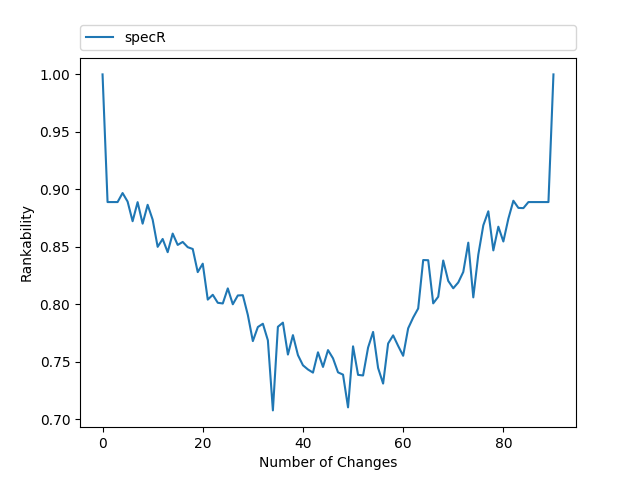
\includegraphics[width=0.5\textwidth]{figures/test_rand_pert_10.png}
&
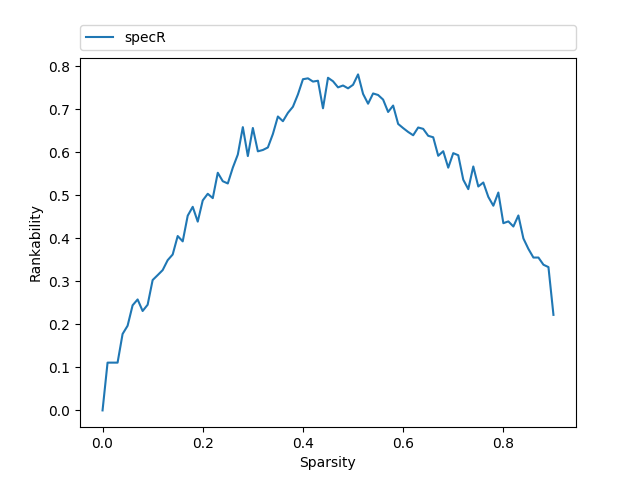
\includegraphics[width=0.5\textwidth]{figures/test_sparse_10.png}
\end{tabular}
\end{frame}

\begin{frame}{Size 20}
\centering
\begin{tabular}{cc}
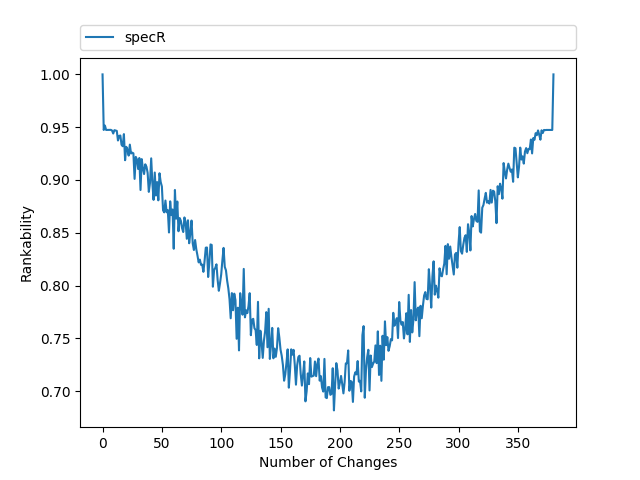
\includegraphics[width=0.5\textwidth]{figures/test_rand_pert_20.png}
&
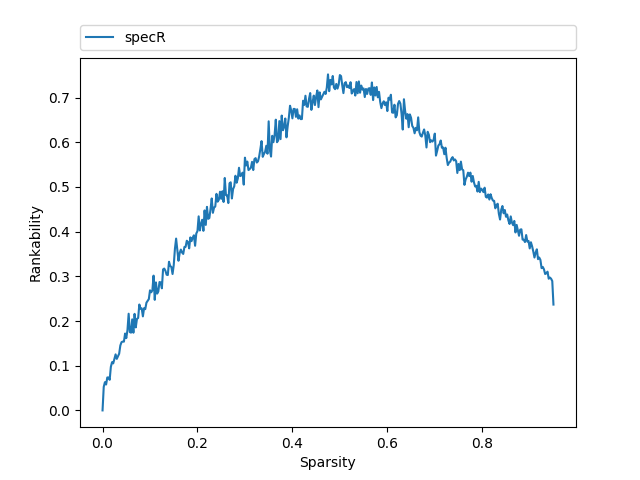
\includegraphics[width=0.5\textwidth]{figures/test_sparse_20.png}
\end{tabular}
\end{frame}

\begin{frame}{Size 30}
\centering
\begin{tabular}{cc}
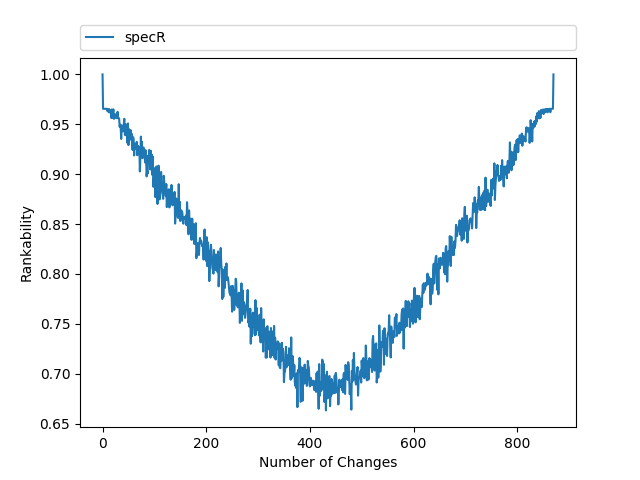
\includegraphics[width=0.5\textwidth]{figures/test_rand_pert_30.png}
&
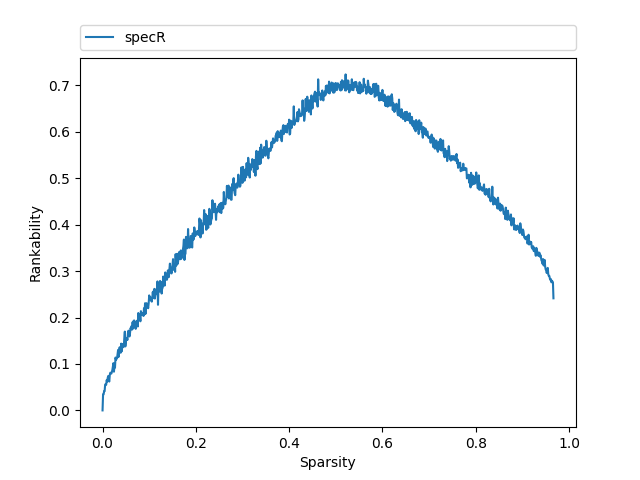
\includegraphics[width=0.5\textwidth]{figures/test_sparse_30.png}
\end{tabular}
\end{frame}

\begin{frame}{Size 40}
\centering
\begin{tabular}{cc}
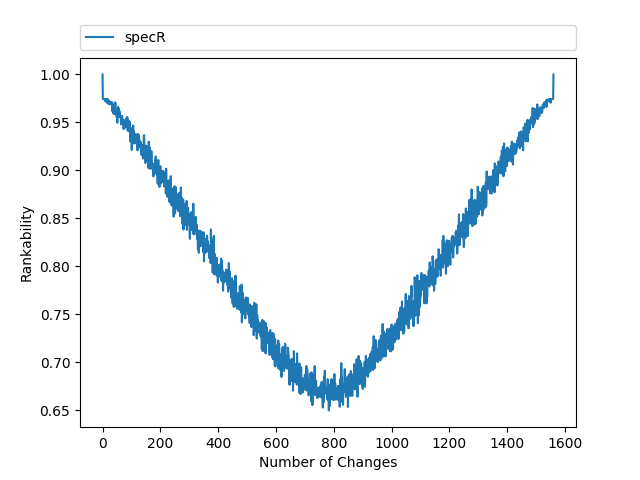
\includegraphics[width=0.5\textwidth]{figures/test_rand_pert_40.png}
&
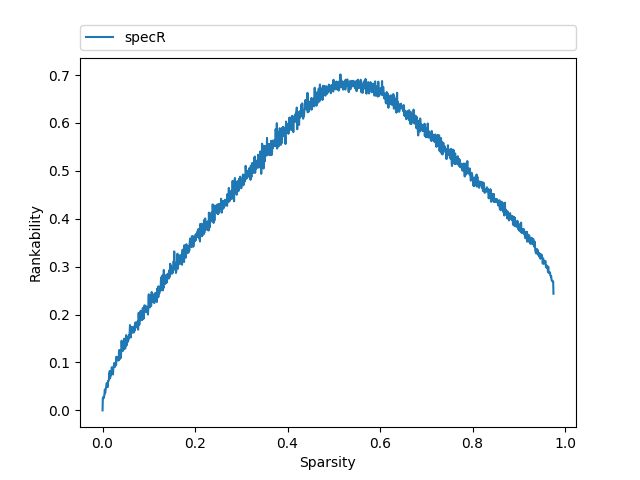
\includegraphics[width=0.5\textwidth]{figures/test_sparse_40.png}
\end{tabular}
\end{frame}

\begin{frame}{Size 50}
\centering
\begin{tabular}{cc}
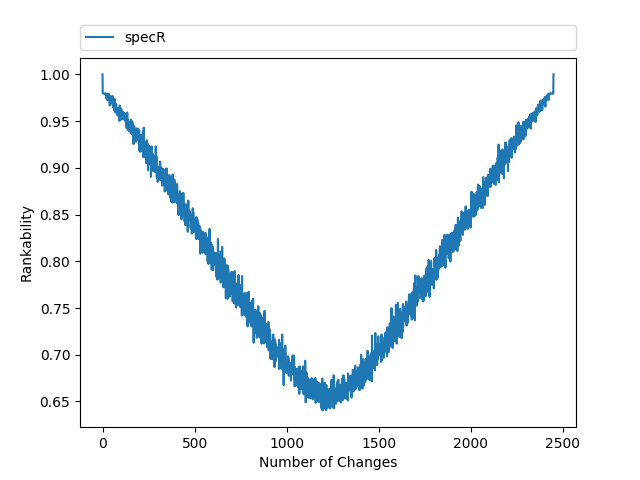
\includegraphics[width=0.5\textwidth]{figures/test_rand_pert_50.png}
&
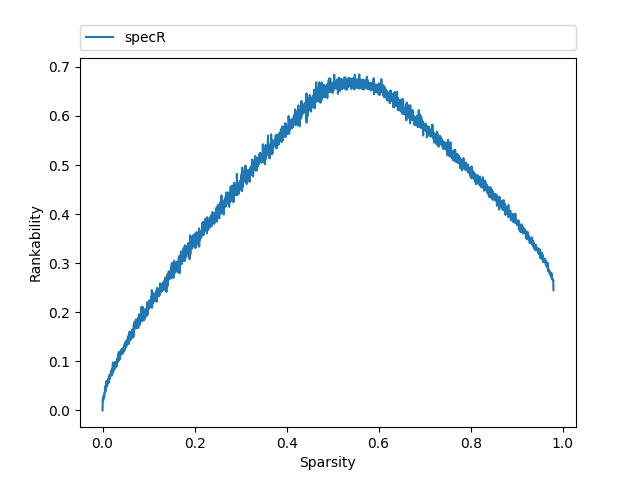
\includegraphics[width=0.5\textwidth]{figures/test_sparse_50.png}
\end{tabular}
\end{frame}

%%%%%%%%%%%%%%%%%%%%%%%%%%%%%%%%%%%%%%%%%%%%%%%%%%%%%%
%								Applications for our Rankability 
%%%%%%%%%%%%%%%%%%%%%%%%%%%%%%%%%%%%%%%%%%%%%%%%%%%%%%
\section{Applications for our Rankability}

\begin{frame}{Tournament Graphs}
A Tournament graph is a directed graph obtained by assigning a direction to each edge in a complete undirected graph.
\vfill
Our rankability measures make sense for data that can be modeled by a tournament (or near-tournament) graph.
\end{frame}

\begin{frame}{Applications}
\begin{itemize}
\item	Sports where each pair of distinct teams play at least one game.
\vfill
\item	Social networks that display dominance relations~\cite{Landau1953}.
\vfill
\item	Preference list voting systems.
\end{itemize}
\end{frame}

\begin{frame}{On Election Voting Systems}
\begin{figure}[H]
\centering
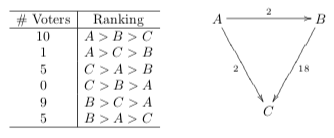
\includegraphics[width=\textwidth]{figures/dodgson-fig1.png}
\caption{Courtesy of~\cite{Ratliff2010}}
\end{figure}
\end{frame}

\begin{frame}{On Election Voting Systems}
\begin{figure}[H]
\centering
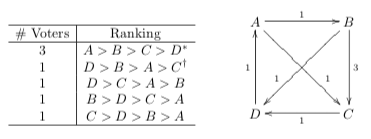
\includegraphics[width=\textwidth]{figures/dodgson-fig2.png}
\caption{Courtesy of~\cite{Ratliff2010}}
\end{figure}
\end{frame}

\begin{frame}{A Different Measure of Rankability}
Model voting preference with binary graph.
\vfill
\begin{theorem}
There exists a Condorcet Winner if and only if the graph Laplacian has an eigenvalue of $(n-1)$ and there exists a vertex with out-degree $(n-1)$. 
\end{theorem}
\end{frame}

\begin{frame}{Results}
Rankability Measure = 1.00
\vfill
\begin{figure}[H]
\centering
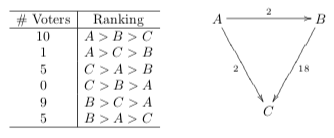
\includegraphics[width=\textwidth]{figures/dodgson-fig1.png}
\caption{Courtesy of~\cite{Ratliff2010}}
\end{figure}
\end{frame}

\begin{frame}{Results}
Rankability Measure = 0.67
\vfill
\begin{figure}[H]
\centering
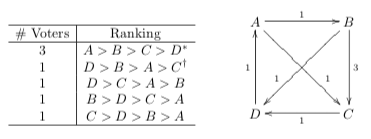
\includegraphics[width=\textwidth]{figures/dodgson-fig2.png}
\caption{Courtesy of~\cite{Ratliff2010}}
\end{figure}
\end{frame}

%%%%%%%%%%%%%%%%%%%%%%%%%%%%%%%%%%%%%%%%%%%%%%%%%%%%%%
%								References 
%%%%%%%%%%%%%%%%%%%%%%%%%%%%%%%%%%%%%%%%%%%%%%%%%%%%%%
\begin{frame}[allowframebreaks]{References}
\bibliographystyle{amsalpha}
\bibliography{../Bibliography}
\end{frame}

\end{document}